\documentclass[12pt]{beamer}
\usetheme{CambridgeUS}
\usepackage[utf8]{inputenc}
\usepackage[german]{babel}
\usepackage[T1]{fontenc}
\usepackage{amsmath}
\usepackage{amsfonts}
\usepackage{amssymb}
\usepackage{graphicx}

\author{Philipp Hörauf und Toni Bartsch}
\title{DIY: Carbonwickelmaschine}

\beamertemplatenavigationsymbolsempty
%\setbeamercovered{transparent} 
%\setbeamertemplate{navigation symbols}{} 
%\logo{}  %Dickbutt!
%\institute{} 
\date{\today} 
\subject{DIY-Vorlesung} 

\begin{document}


\begin{frame}
\titlepage
\end{frame}


\begin{frame}
\tableofcontents
\end{frame}

\section{Ziel des Projektes}
\begin{frame}{Was war das Ziel?}
Eigenbau einer Carbonwickelmaschine aus Normteilen und selbst Designtem.\newline
\vspace{0.5cm}


geplante Eckdaten der Maschine:
\begin{itemize}
	\item Maximale Wickellänge 1200\,mm
	\item Größter Durchmesser 250\,mm
	\item Verarbeitung von Carbon- und Glasfasern
	\item Wickelvorgang PC-kontrolliert
	\item Möglichst kostengünstiger Aufbau
\end{itemize}

\end{frame}


\begin{frame}{Projektstatus}
\section{Aktueller Projektstatus}
Problem: Defekt der Frässpindel\newline
Selbst gefräste Teile die für die Maschine notwendig sind konnten nicht hergestellt werden.

\begin{figure}
	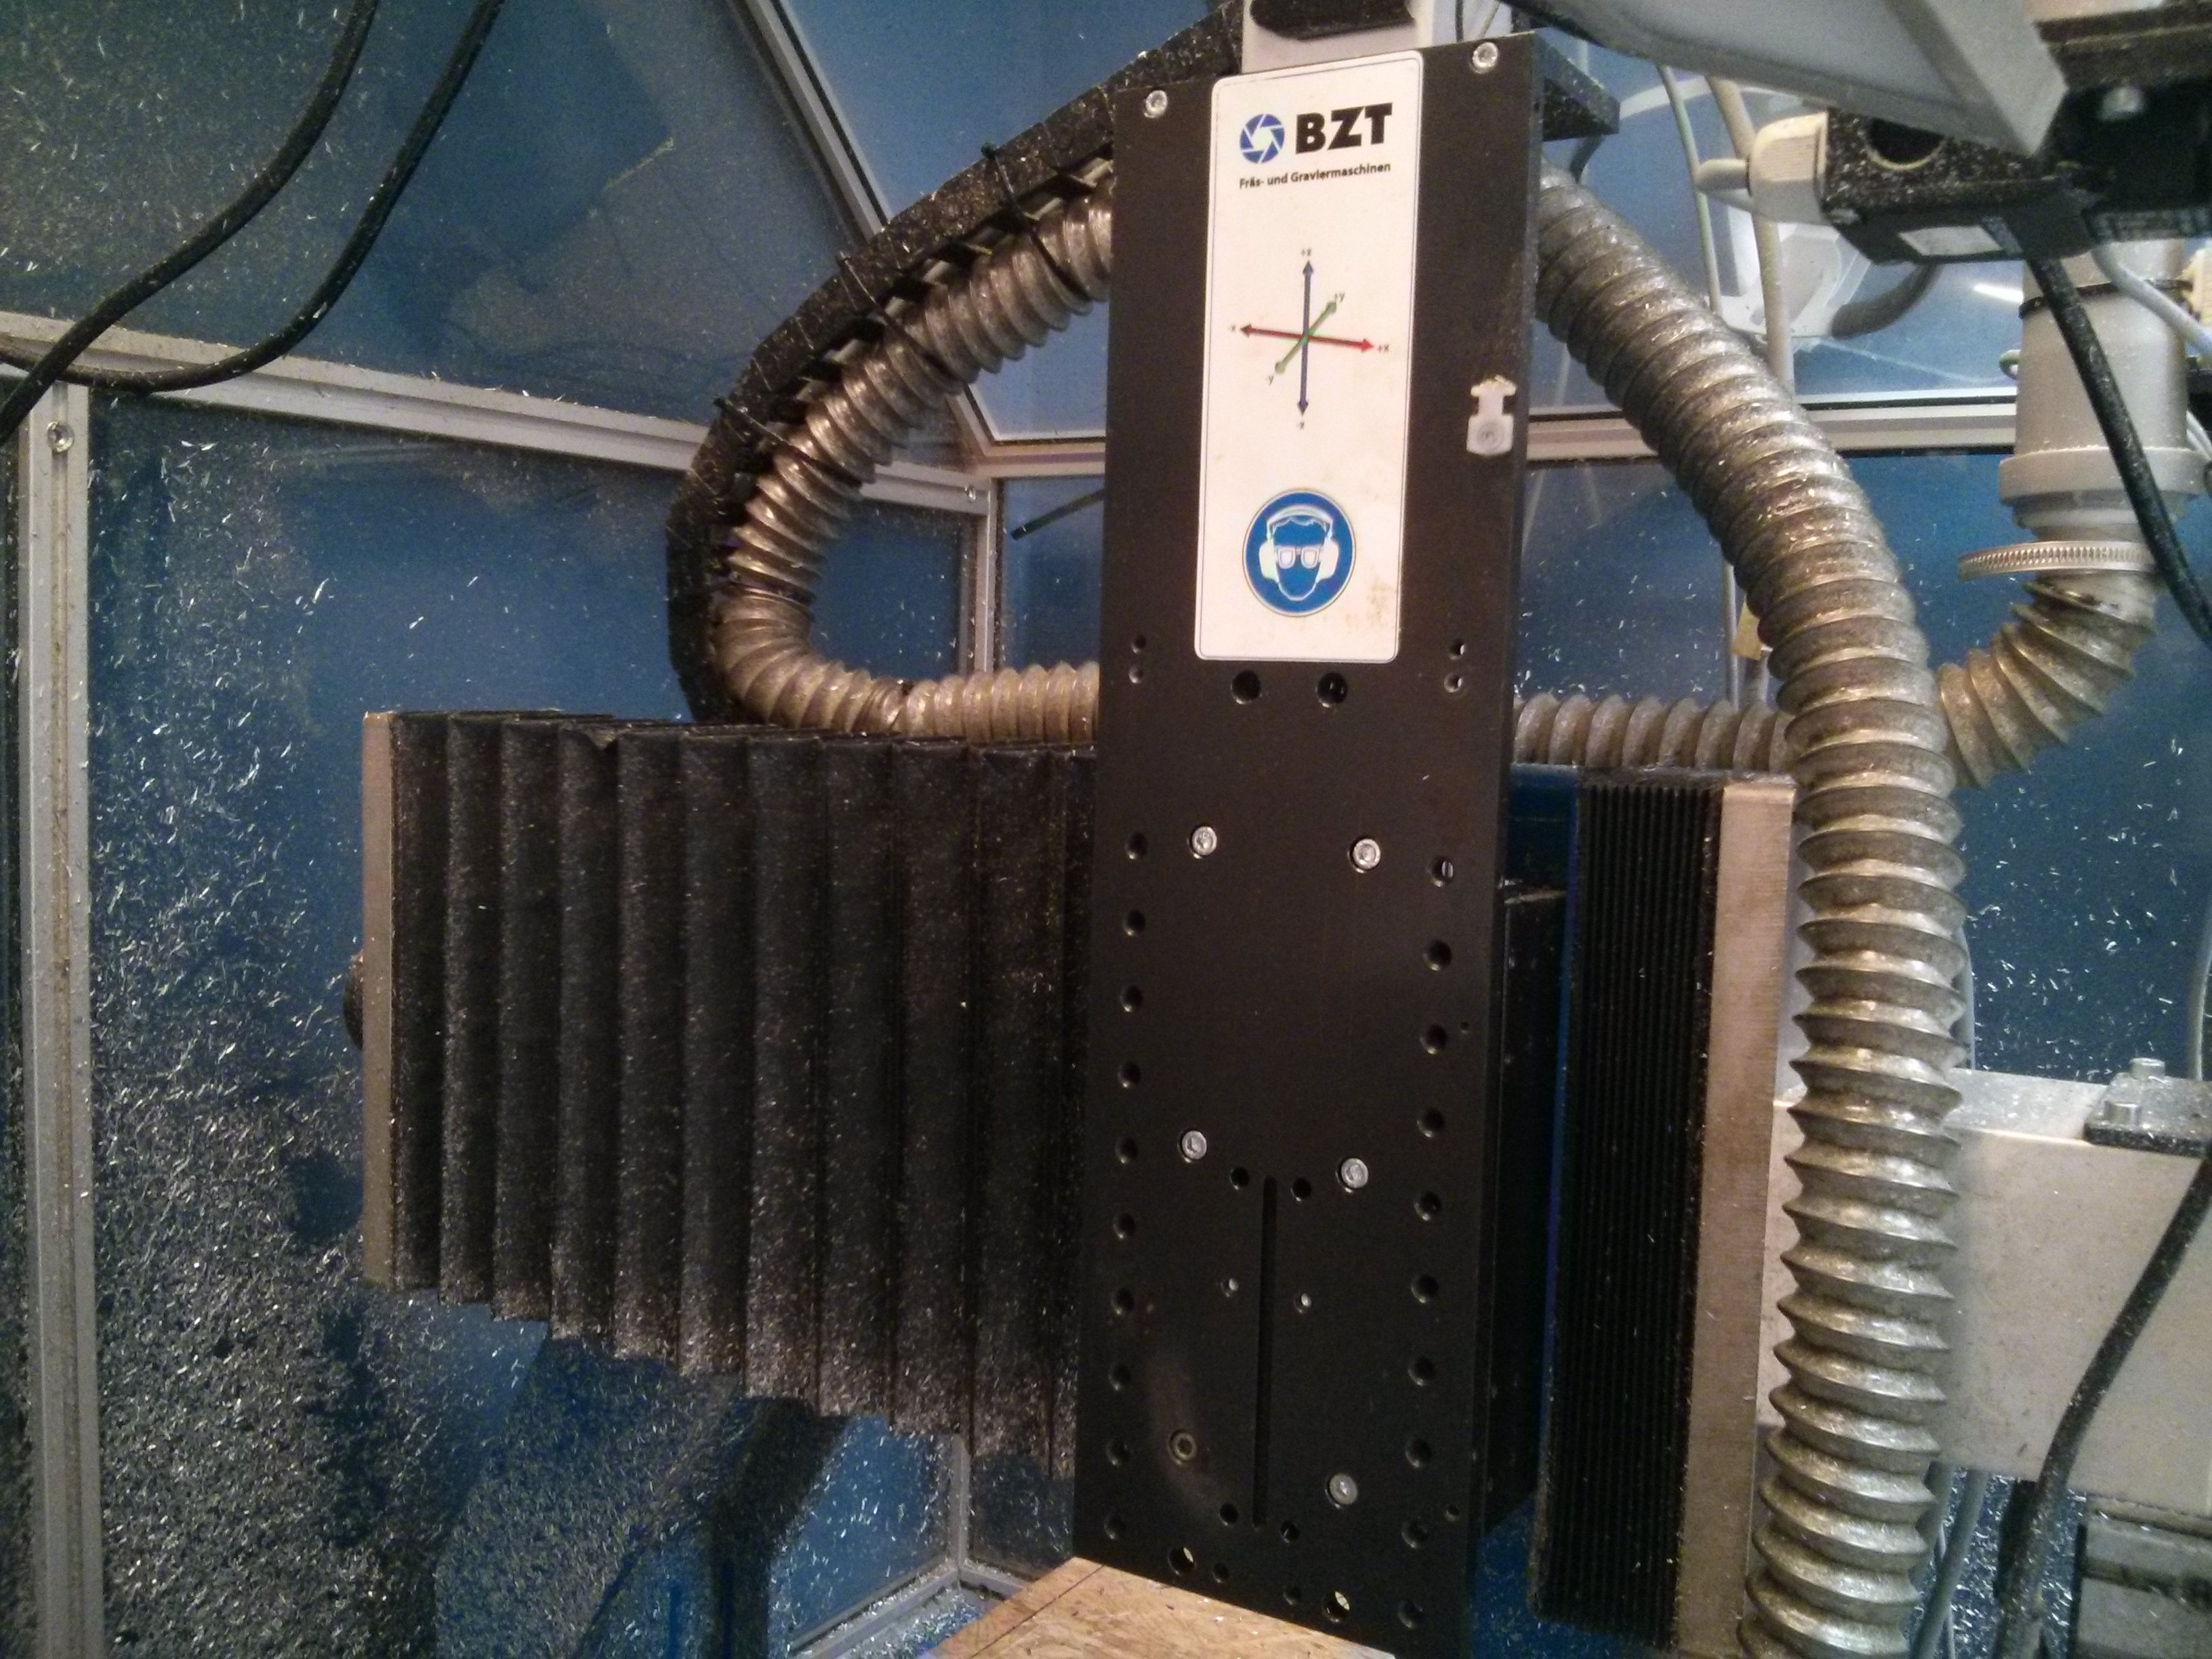
\includegraphics[width=6cm]{bilder/fraese_defekt.jpg}
	\caption{Fräse ohne Frässpindel}
\end{figure}

\end{frame}


\subsection{Mechanischer Aufbau}
\begin{frame}{Mechanischer Aufbau}
3D Modell der Wickelmaschine in Siemens NX
\begin{figure}
	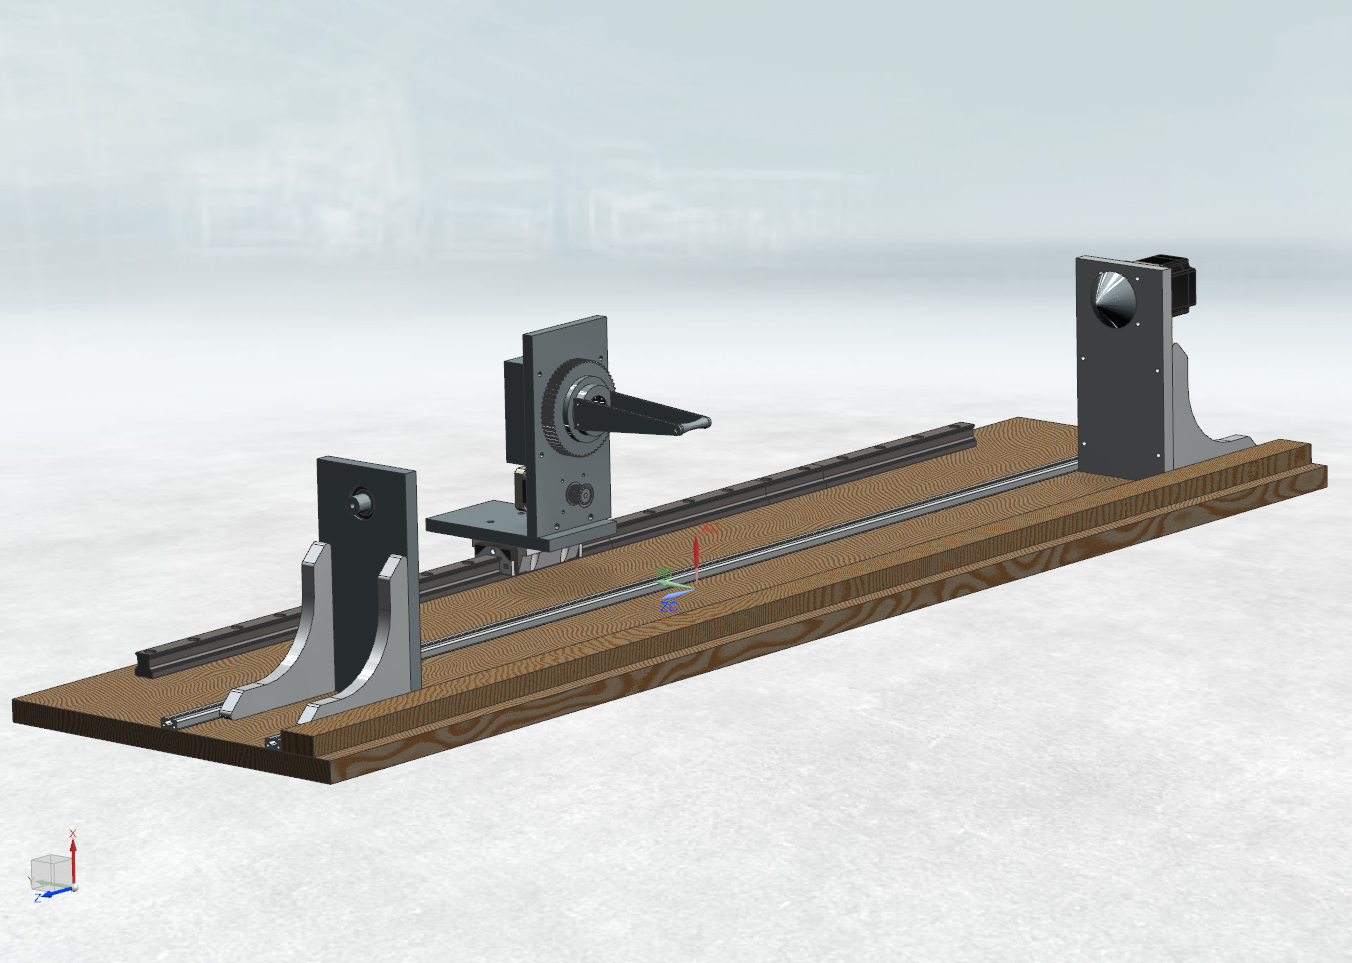
\includegraphics[width=8cm]{NX_Screenshots/gesamt3.png}
	\caption{3D-Modell der Wickelmaschine}
\end{figure}
\end{frame}

\begin{frame}
\begin{figure}
	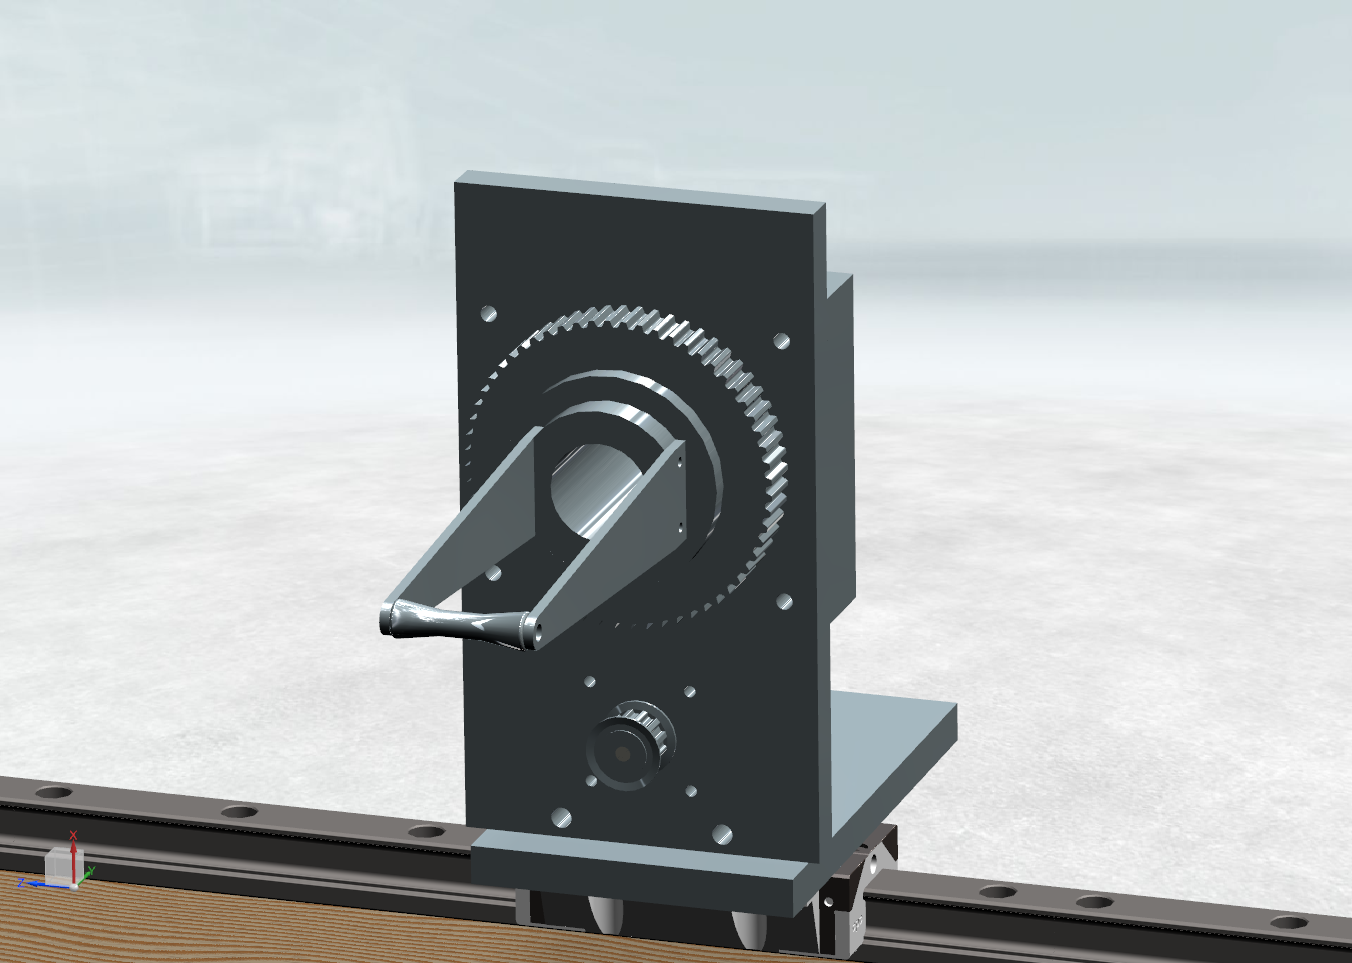
\includegraphics[width=10cm]{NX_Screenshots/arm_vorne.png}
	\caption{Detailansicht Dreharm}
\end{figure}
\end{frame}


\begin{frame}{Software}
\subsection{Software}
Entwickelte Software zur Erzeugung von G-Code zur Ansteuerung der Maschine

\begin{figure}
	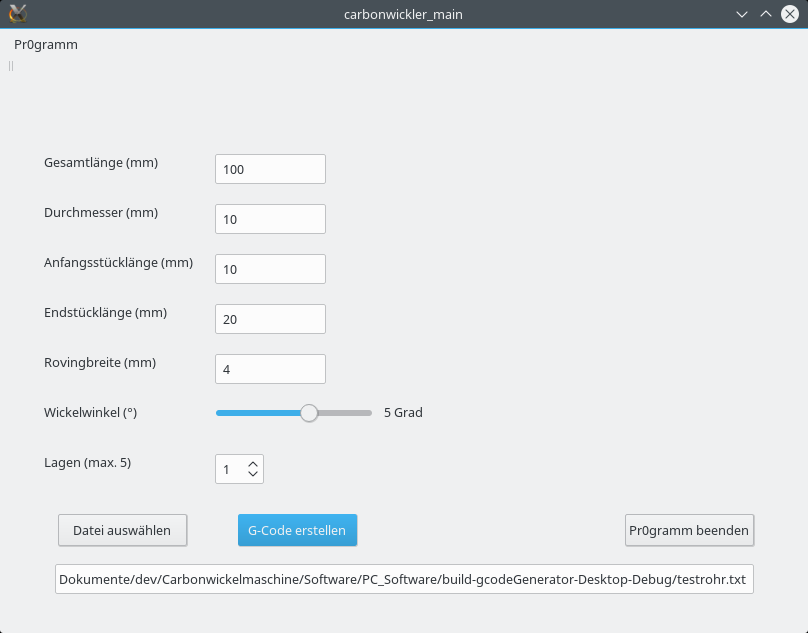
\includegraphics[width=7cm]{bilder/carbowickler_software.png}
	\caption{Screenshot des G-Codegenerators}
\end{figure}
\end{frame}

\begin{frame}{Ausblick}
\section{Ausblick}
\begin{center}
Fertigstellung des Projektes,\\sobald die Fräse wieder einsatzbereit ist.
\end{center} 
\end{frame}


\end{document}